\chapter{Wymagania i narzędzia}
\label{ch:wymagania-i-narzedzia}

\paragraph{}
Tworzona aplikacja ma ułatwić użytkownikowi zarządzanie lokalizatorami, kierowcami i pojazdami jednocześnie oraz pozwalać na wyświetlanie tras poszczególnych kierowców i pojazdów. Wymagania aplikacji należy podzielić na funkcjonalne i niefunkcjonalne. Przyjrzyjmy się w pierwszej kolejności wymaganiom funkcjonalnym. Poniżej wypisano przewidziane przypapadki użycia programu.

\paragraph{}
Dla niezalogowanego użytkownika (przedstawia je również diagram widoczny na rys 3.1):

\begin{itemize}
\item Rejestracja - gdy użytkownik wchodzi na stronę aplikacji, może się zarejestrować, czyli stworzyć bezpłatne konto, które będzie przypisane do podanego przez niego w formularzu rejestracji adresu email
\item Logowanie - w przypadku uprzedniej rejestracji w systemie, użytkownik może zalogować się na istniejące konto
\end{itemize}

\paragraph{}
Dla zalogowanego użytkownika (przedstawia je również diagram widoczny na rys 3.2):
\begin{itemize}
\item Dodanie obiektu
	\begin{itemize}
	\item Dodanie kierowcy - użytkownik ma możliwość dodania kierowcy do swojego konta, podając ich imię oraz nazwisko
	\item Dodanie pojazdu - pozwala dodać pojazd do konta poprzez podanie jego marki, modelu, numeru rejestracyjnego oraz numeru VIN
	\item Dodanie lokalizatora - w ten sposób użytkownik może dodać posiadane lokalizatory TK108 do swojego konta, podając jego nazwę, numer seryjny oraz typ
	\end{itemize}
\item Dodanie powiązania
\begin{itemize}
	\item Dodanie kierowcy pojazdu - ten przypadek umożliwia powiązanie kierowcy z pojazdem w podanym przez użytkownika okresie czasu 
	\item Dodanie lokalizatora w pojeździe - działa na takiej zasadzie, jak powyższy podpunkt, umożliwia powiązanie lokalizatora z pojazdem w danym okresie czasu
\end{itemize}
\item Wyświetlenie trasy
\begin{itemize}
	\item Wyświetlenie trasy kierowcy - użytkownik może wyświetlić na mapie trasę przebytą przez danego kierowcę w wybranym przez siebie okresie czasu
	\item Wyświetlenie trasy pojazdu - analogicznie do powyższego przypadku, możliwość wyświetlenia trasy pokonanej przez pojazd w danym czasie
\end{itemize}
\item Usunięcie obiektu
\begin{itemize}
	\item Usunięcie kierowcy - powoduje usunięcie istniejącego kierowcy z systemu
	\item Usunięcie pojazdu - daje możliwość usunięcia wybranego pojazdu z aplikacji
	\item Usunięcie lokalizatora - podobnie do powyższych, skutkuje usunięciem danego lokalizatora
\end{itemize}
\item Usunięcie powiązania
\begin{itemize}
	\item Usunięcie kierowcy pojazdu - usuwa czasowe powiązanie kierowcy oraz pojazdu
	\item Usunięcie lokalizatora w pojeździe - analogicznie, użytkownik może się w ten sposób pozbyć powiązania lokalizatora z pojazdem z danego okresu czasu
\end{itemize}
\item Usunięcie trasy z mapy
\begin{itemize}
	\item Usunięcie trasy kierowcy - powoduje zniknięcie z mapy trasy kierowcy z danego okresu czasu
	\item Usunięcie trasy pojazdu - pozwala usunąć z mapy wcześniej wyświetloną trasę pojazdu 
\end{itemize}
\end{itemize}


\paragraph{}
Przejdźmy teraz do wymagań niefunkcjonalnych:

\begin{itemize}
	\item Niskie wymagania systemowe - aplikacja powinna być dostępna dla każdego urządzenia posiadającego przeglądarkę internetową oraz dostęp do internetu. W tym celu wymagane jest, aby program był aplikacją przeglądarką.
	\item Skalowalność interfejsu użytkownika - wymagane jest, aby program był dostosowany do różnej wielkości oraz rozdzielczości ekranów. Użytkowanie aplikacji na smartfonie powinno być równie sprawne i nie sprawiające problemów, jak podczas korzystania z komputera stacjonarnego lub laptopa.
	\item Prosta obsługa - ze względu na duże i zróżnicowane grono potencjalnych użytkowników, założono, iż aplikacja będzie możliwie jak najmniej skomplikowana w obsłudze. Dostęp do każdej funkcji programu powininem być możliwy przy wykonaniu minimalnej ilości kliknięć myszy (lub ekranu w przypadku urządzeń dotykowych), nieprzekraczającej trzech.
\end{itemize}

\begin{figure}
\centering
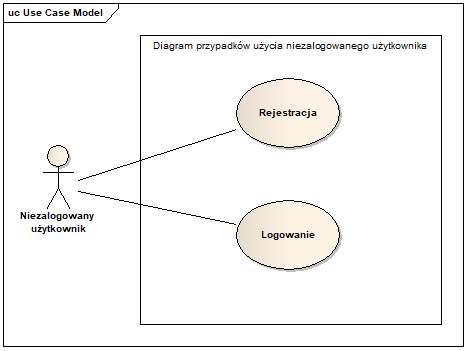
\includegraphics[width=0.6\textwidth]{./graf/Przypadki_uzycia_niezalogowany.png}
\caption{Diagram przypadków użycia niezalogowanego użytkownika.}
\label{fig:3.1}
\end{figure}

\begin{figure}
\centering
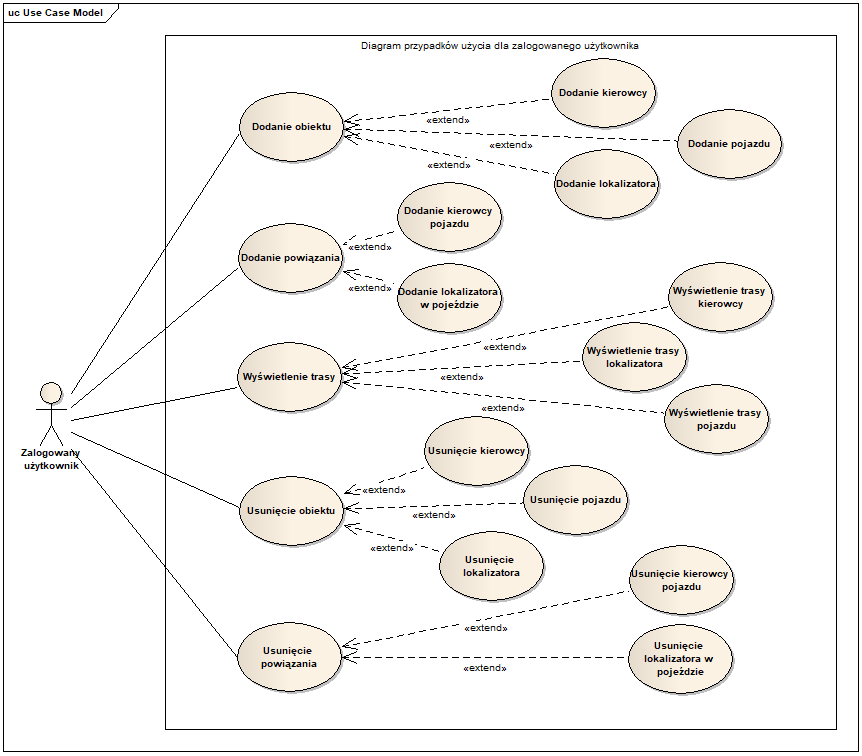
\includegraphics[width=1\textwidth]{./graf/Przypadki_uzycia_zalogowany.png}
\caption{Diagram przypadków użycia zalogowanego użytkownika.}
\label{fig:3.2}
\end{figure}

\paragraph{}
Aby przystąpić do tworzenia aplikacji, należało przygotować odpowiednie narzędzia. W pierwszej kolejności zakupiono lokalizator TK108 oraz kartę SIM, aby możliwe było uruchomienie i skonfigurowanie urządzenia. Kolejnym etapem było zainstalowanie niezbędnego oprogramowania do edycji kodu źródłowego aplikacji. Do części funkcjonalnej został wykorzystany Intellij Idea wydawcy JetBrains. Ten program jest zaawansowanym, wieloplatformowym środowiskiem programistycznym, posiadającym dużą ilość wbudowanych narzędzi, jak również obsługującym wiele bibliotek i platform programistycznych, takich jak Spring Boot. Hibernate oraz JPA również są wspierane przez Intellij. Są to narzędzia, które potrafią powiązać kod aplikacji z bazą danych, co znacznie uprości rozwijanie programu. W kontekście bazy danych, potrzebne było oprogramowanie, które będzie w stanie obsługiwać zapytania kierowane do bazy danych - na początku do stworzenia bazy, poszczególnych tabel, a w przyszłości do eliminiowania ewentualnych błędów oraz do testowania aplikacji. Przechodząc do interfejsu użytkownika, a zatem do kodu w języku TypeScript z zastosowaniem biblioteki React, wybrano Microsoft Visual Studio Code, który jest powszechnie używany przez programistóW w tym celu, ze względu na odpowiednie wsparcie języków i bibliotek typowych do tworzenia wizualnej części aplikacji. Ostatnim elementem jest narzędzie do systemu kontroli wersji. Dzięki temu postępy w pracy będą zabezpieczone. Nie mniej jednak, to nie jedyny atut. W przypadku błędów aplikacji spowodowanych zmianami w kodzie źródłowym, zlokalizowanie ich przyczyny będzie znacznie ułatwione. Wybrano system Git, gdyż jest on najpopularniejszą opcją, a co za tym idzie, jest obsługiwany przez niemal każde oprogramowanie programistyczne, lecz to nie wszystko. Należy również dokonać wyboru platformy hostingowej, która będzie przechowywała repozytorium Git. W tym celu skorzystano z GitHuba, będącego jedną z najbardziej powszechnych opcji. Jest on także wspierany przez większość środowisk programistycznych. 

%\begin{itemize}
%\item wymagania funkcjonalne i niefunkcjonalne
%\item przypadki użycia (diagramy UML) -- dla prac, w których mają zastosowanie
%\item opis narzędzi, metod eksperymentalnych, metod modelowania itp.
%\item metodyka pracy nad projektowaniem i implementacją -- dla prac, w których ma to zastosowanie
%\end{itemize}
